
%(BEGIN_QUESTION)
% Copyright 2008, Tony R. Kuphaldt, released under the Creative Commons Attribution License (v 1.0)
% This means you may do almost anything with this work of mine, so long as you give me proper credit

The following storage vessel holds water.  The hydrostatic-pressure level transmitter is located 5 feet below the bottom of the vessel, and the desired level measurement range is 8 feet to 12 feet:

$$\includegraphics[width=15.5cm]{i00257x01.eps}$$

Assuming a pneumatic transmitter with an output range of 3 PSI to 15 PSI, and a calibration accuracy of +/- 1\% of span, complete the following calibration table for the transmitter:

% No blank lines allowed between lines of an \halign structure!
% I use comments (%) instead, so that TeX doesn't choke.

$$\vbox{\offinterlineskip
\halign{\strut
\vrule \quad\hfil # \ \hfil & 
\vrule \quad\hfil # \ \hfil & 
\vrule \quad\hfil # \ \hfil & 
\vrule \quad\hfil # \ \hfil & 
\vrule \quad\hfil # \ \hfil & 
\vrule \quad\hfil # \ \hfil \vrule \cr
\noalign{\hrule}
%
% First row
Process & Percent of & $\Delta$ pressure & Output signal & Output signal & Output signal \cr
%
% Another row
level (ft) & span (\%) & sensed ("W.C) & ideal (PSI) & min. (PSI) & max. (PSI) \cr
%
\noalign{\hrule}
%
% Another row
  & 0 &  &  &  &  \cr
%
\noalign{\hrule}
%
% Another row
  & 10 &  &  &  &  \cr
%
\noalign{\hrule}
%
% Another row
  & 25 &  &  &  &  \cr
%
\noalign{\hrule}
%
% Another row
  & 50 &  &  &  &  \cr
%
\noalign{\hrule}
%
% Another row
  & 75 &  &  &  &  \cr
%
\noalign{\hrule}
%
% Another row
  & 90 &  &  &  &  \cr
%
\noalign{\hrule}
%
% Another row
  & 100 &  &  &  &  \cr
%
\noalign{\hrule}
} % End of \halign 
}$$ % End of \vbox

\underbar{file i00257}
%(END_QUESTION)





%(BEGIN_ANSWER)

% No blank lines allowed between lines of an \halign structure!
% I use comments (%) instead, so that TeX doesn't choke.

$$\vbox{\offinterlineskip
\halign{\strut
\vrule \quad\hfil # \ \hfil & 
\vrule \quad\hfil # \ \hfil & 
\vrule \quad\hfil # \ \hfil & 
\vrule \quad\hfil # \ \hfil & 
\vrule \quad\hfil # \ \hfil & 
\vrule \quad\hfil # \ \hfil \vrule \cr
\noalign{\hrule}
%
% First row
Process & Percent of & $\Delta$ pressure & Output signal & Output signal & Output signal \cr
%
% Another row
level (ft) & span (\%) & sensed ("W.C) & ideal (PSI) & min. (PSI) & max. (PSI) \cr
%
\noalign{\hrule}
%
% Another row
8 & 0 & 156 & 3 & 2.88 & 3.12 \cr
%
\noalign{\hrule}
%
% Another row
8.4 & 10 & 160.8 & 4.2 & 4.08 & 4.32 \cr
%
\noalign{\hrule}
%
% Another row
9 & 25 & 168 & 6 & 5.88 & 6.12 \cr
%
\noalign{\hrule}
%
% Another row
10 & 50 & 180 & 9 & 8.88 & 9.12 \cr
%
\noalign{\hrule}
%
% Another row
11 & 75 & 192 & 12 & 11.88 & 12.12 \cr
%
\noalign{\hrule}
%
% Another row
11.6 & 90 & 199.2 & 13.8 & 13.68 & 13.92 \cr
%
\noalign{\hrule}
%
% Another row
12 & 100 & 204 & 15 & 14.88 & 15.12 \cr
%
\noalign{\hrule}
} % End of \halign 
}$$ % End of \vbox

%(END_ANSWER)





%(BEGIN_NOTES)


%INDEX% Calibration: table, level transmitter
%INDEX% Measurement, level: calibration table
%INDEX% Measurement, level: hydrostatic pressure (suppressed zero)

%(END_NOTES)


